\documentclass[centertitle]{notes}
\usepackage{lipsum}

\coursetitle{An Introduction to Advanced Topics}
\subtitle{Lecture Notes}
\coursecode{am224}
\professor{Khabib Nurmagomedov\thanks{Let's talk now.}}
\scribe{
  Matthew Nazari\titlehref[mailto:matthewnazari@college.harvard.edu]{matthewnazari@college}[email]
  \and
  Bella Tarantino\titlehref[mailto:bellatarantino@college.harvard.edu]{bellatarantino@college}[email]
}
\place{Harvard University}
\flag{This is a example document. Ut lorem lorem, interdum eu, tincidunt sit amet, laoreet vitae, arcu.}
\date{31}{2}{2024}

\begin{document}


  \section{Introduction}
  \lipsum[1]
  \marginpar{Ut lorem lorem, interdum eu, tincidunt sit amet, laoreet vitae, arcu. Aenean faucibus pede eu ante.}
  \lipsum[2]
  \subsection{This is a subsection}
  \lipsum[3]
  \begin{marginfig}[Nunc elementum fermentum wisi. Aenean placerat\protect\footnotemark]
    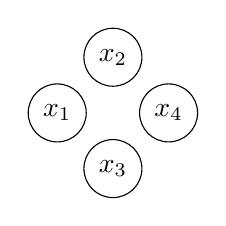
\begin{tikzpicture}[main/.style = {draw, circle}]
      \node[main] (1) {$x_1$};
      \node[main] (2) [above right of=1] {$x_2$};
      \node[main] (3) [below right of=1] {$x_3$}; 
      \node[main] (4) [above right of=3] {$x_4$};
    \end{tikzpicture}
  \end{marginfig}
  \footnotetext{Donec eu purus.Quisque vehicula, urna sed ultricies auctor.}
  \lipsum[4-5]
  \begin{definition}[statistical model]
    A {\italics statistical model} is a family of probability distributions indexed by a parameter $\theta \in \Theta$ where $\Theta$, the {\italics parameter space}, is the set of all allowable parameter values.
  \end{definition}
  \lipsum[6]
  \marginpar{Suspendisse vel felis. Ut lorem lorem, interdum eu, tincidunt sit amet, laoreet vitae, arcu.Aenean faucibus pede eu ante.}
  \subsection{Still introducting things}
  \lipsum[7]


  \section{A continuation}
  \lipsum[8]
  \begin{proposition}
    It is given that if $\E[\theta]$ exists, then $\MSE(\hat\theta) = \E[\hat\theta - \theta]^2$.
  \end{proposition}
  \begin{theorem}[Theorem]
    The mean square error of an estimator $\hat\theta$ is the variance plus the square of the bias: $$\MSE(\hat\theta) = \Var(\hat\theta) + (\bias(\hat\theta))^2.$$
  \end{theorem}
  \begin{proof} This theorem directly follows from the definition of variance:
    \begin{align*}
      \MSE(\hat\theta) &= \E[\hat\theta - \theta]^2 \\
                       &= \Var(\hat\theta - \theta) + (\E[\hat\theta - \theta])^2 \\
                       &= \Var(\hat\theta - \theta) + (\E[\hat\theta] - \theta)^2 \\
                       &= \Var(\hat\theta) + (\bias(\hat\theta))^2.
    \end{align*}
  \end{proof}
  \marginpar[2em]{\it{Caution.} Nulla facilisi. Pellentesque eget lectus. Proin eu metus. Sed porttitor.}
  \lipsum[9]\footnote{Nulla facilisi. Pellentesque eget lectus. Proin eu metus. Sed porttitor.}
  \begin{example}[This is an example]
    The family of all normal distributions, $\{\N(\mu, \sigma^2) : \mu \in \R, \sigma > 0\}$, is a 2-dimensional parametric model where $\Theta = \{\theta : \theta \in \R \times \R^+\}$. But models don't have to be named distributions. Suppose we have a population of cats and dogs, and we are studying the weight $Y$ of a random animal from the population. Let $p$ be the proportion of cats in the population. Suppose the weight of a random cat and a random dog is $\N(\mu_1, {\sigma_1}^2)$ and $\N(\mu_2, {\sigma_2}^2)$ respectively. Then by the LOTP, the CDF of $Y$ is 
    \begin{align*}
      F_Y(y) = P(Y \leq y) &= P(Y \leq y \mid \t{cat})P(\t{cat}) + P(Y \leq y \mid \t{dog})P(\t{dog}) \\
                          &= p\,\Phi(\frac{y - \mu_1}{\sigma_1}) + (1-p)\,\Phi(\frac{y - \mu_2}{\sigma_2}).
    \end{align*}
    The CDF of $Y$ depends on the parameter $\theta = (p, \mu_1, \sigma_1, \mu_2, \sigma_2)$, so we write it as as $F_Y(y \mid \theta)$. Our model, therefore, is the collection of all CDFs $F_Y(y \mid \theta)$ indexed by $\theta \in \Theta =\{\theta : \theta \in [0, 1] \times \R \times \R^+ \times \R \times \R^+\}$. This is a 5-dimensional parametric model.
  \end{example}
  \lipsum[10]
  \begin{note}
    liquam vestibulum fringilla lorem. Sed neque lectus, consectetuerat, consectetuer sed, eleifend ac, lectus. Nulla facilisi. Pellentesque eget lectus. Proin eu metus.Sed porttitor. In hac habitasse platea dictumst. Suspendisse eu lectus. Ut mi mi, lacinia sit amet, placerat et.
  \end{note}
  \lipsum[11]
  \begin{fig}[Ut lorem lorem, interdum eu, tincidunt sit amet, laoreet vitae, arcu. Aenean faucibus pede eu ante. Amet, laoreet vitae, arcu.]%
    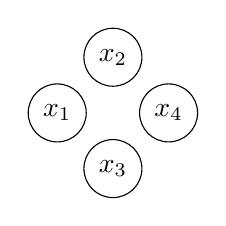
\begin{tikzpicture}[main/.style = {draw, circle}]
      \node[main] (1) {$x_1$};
      \node[main] (2) [above right of=1] {$x_2$};
      \node[main] (3) [below right of=1] {$x_3$}; 
      \node[main] (4) [above right of=3] {$x_4$};
    \end{tikzpicture}
  \end{fig}
  \lipsum[12-13]
  \subsection{Planets, moons, and stars}
  \lipsum[14]
  \begin{remark}
    Etiam euismod. Fusce facilisis lacinia dui. Suspendisse potenti. In mi erat, cursus id, nonummy sed, ullamcorper eget, sapien.
  \end{remark}
  \lipsum[14]


  \section{A Final Section}
  \lipsum[15]
  \subsection{Closing Remarks}
  \lipsum[16]

  
\end{document}

